\documentclass[12pt,a4paper]{article}
\usepackage[utf8]{inputenc}
\usepackage[T2A]{fontenc}
\usepackage[russian]{babel}
\usepackage{setspace}
\usepackage{geometry}
\usepackage{graphicx}
\usepackage{booktabs}
\usepackage{indentfirst}
\usepackage{multirow}
\usepackage{amsmath}
\usepackage{float}
\usepackage{hyperref}
\geometry{left=30mm,right=15mm,top=20mm,bottom=20mm}

\pagestyle{plain}
\setcounter{page}{1}

% --- Макросы с числами (меняем тут - обновляется везде) ---
\newcommand{\repvggAcc}{93.88}
\newcommand{\resnetAcc}{91.39}
\newcommand{\vggAcc}{93.46}
\newcommand{\repvggParams}{7.84}
\newcommand{\repvggDeployParams}{7.04}
\newcommand{\resnetParams}{0.27}
\newcommand{\vggParams}{14.72}
\newcommand{\repvggFlops}{984.8}
\newcommand{\repvggDeployFlops}{883.0}
\newcommand{\repvggInfTrain}{6.3}
\newcommand{\repvggInfDeploy}{1.7}
\newcommand{\repvggSpeedup}{3.7}
% Ablation (100 эпох)
\newcommand{\ablFull}{93.88}
\newcommand{\ablNoId}{93.55}
\newcommand{\ablNoOne}{93.29}
\newcommand{\ablOnlyThree}{93.38}
% Cutout
\newcommand{\cutoutAcc}{94.90}
% FLOPs baseline
\newcommand{\resnetFlops}{82.8}
\newcommand{\vggFlops}{629.1}
\newcommand{\resnetInf}{1.7}
\newcommand{\vggInf}{1.3}

\begin{document}
\thispagestyle{empty}
\onehalfspacing

\begin{center}
ПРАВИТЕЛЬСТВО РОССИЙСКОЙ ФЕДЕРАЦИИ\\[0.5em]
ФЕДЕРАЛЬНОЕ ГОСУДАРСТВЕННОЕ АВТОНОМНОЕ ОБРАЗОВАТЕЛЬНОЕ\\
УЧРЕЖДЕНИЕ ВЫСШЕГО ОБРАЗОВАНИЯ\\[0.5em]
<<НАЦИОНАЛЬНЫЙ ИССЛЕДОВАТЕЛЬСКИЙ УНИВЕРСИТЕТ\\
<<ВЫСШАЯ ШКОЛА ЭКОНОМИКИ>>\\
\end{center}

\vspace{10mm}

\begin{center}
Факультет компьютерных наук\\
Образовательная программа <<Искусственный интеллект>>\\
\end{center}

\vspace{15mm}

\begin{center}
\textbf{\Large Воспроизведение результатов статьи}\\[0.7em]
\textbf{\Large <<RepVGG: Making VGG-style ConvNets Great Again>>}\\
\end{center}

\vspace{10mm}

\begin{center}
Отчет об исследовательском проекте\\
\end{center}

\vspace{20mm}

\begin{flushright}
\begin{minipage}{0.45\textwidth}
Выполнил студент:\\
Власов Владислав Сергеевич\\
\end{minipage}
\end{flushright}

\vfill

\begin{center}
Москва 2026 г.
\end{center}

\clearpage

%______________________________________________________
% АННОТАЦИЯ

\begin{center}
\textbf{АННОТАЦИЯ}
\end{center}

Воспроизведены ключевые результаты статьи RepVGG~[1] на CIFAR-10. Реализована архитектура RepVGG-A0 со структурной репараметризацией: при обучении блок содержит три параллельные ветки ($3\times3$, $1\times1$, identity), при инференсе они сливаются в одну свёртку $3\times3$ без потери точности. Проведены четыре группы экспериментов: верификация слияния весов, сравнение с ResNet-20 и VGG-16, ablation по веткам, влияние аугментации Cutout. Обучение и логирование выполнены на NVIDIA RTX~3070 с фиксацией метрик в Weights~\&~Biases.

\clearpage
\tableofcontents
\clearpage

%______________________________________________________
% ВВЕДЕНИЕ

\section{Введение}

Современные свёрточные архитектуры повышают точность за счёт усложнения топологии: skip-connections (ResNet), плотные связи (DenseNet), автоматически найденные графы (NAS). Побочный эффект - замедление инференса: разветвления снижают утилизацию GPU, увеличивают пиковый расход памяти и усложняют развёртывание.

Ding~et~al.~[1] разделили тренировочную и инференс-архитектуру. При обучении каждый блок содержит три ветки, что расширяет пространство оптимизации. При деплое ветки сливаются в единственную свёртку $3\times3$ через структурную репараметризацию, и модель становится plain-цепочкой вида conv-relu без разветвлений.

Оригинальная статья приводит результаты только для ImageNet, поэтому прямое сравнение наших чисел с авторскими невозможно. Цель работы - воспроизвести ключевую идею RepVGG (структурную репараметризацию) на CIFAR-10, проверить её корректность, оценить вклад отдельных веток и сравнить результат с ResNet-20~[2] и VGG-16~[3] в одинаковых условиях обучения.

%______________________________________________________
% ОБЗОР СТАТЬИ

\section{Обзор архитектуры RepVGG}

\subsection{Тренировочный блок}

При обучении RepVGG-блок суммирует три параллельные ветки:
\begin{itemize}
    \item свёртка $3\times3$ + BatchNorm,
    \item свёртка $1\times1$ + BatchNorm,
    \item identity + BatchNorm (при $C_{\text{in}} = C_{\text{out}}$, stride $= 1$).
\end{itemize}

Выход до нелинейности:
\[
y = \text{BN}_3(\text{Conv}_{3\times3}(x)) \;+\; \text{BN}_1(\text{Conv}_{1\times1}(x)) \;+\; \text{BN}_{\text{id}}(x)
\]

Identity-ветка играет роль, аналогичную residual connection в ResNet, - облегчает распространение градиентов. Ветка $1\times1$ расширяет множество достижимых функций при обучении, но исчезает при слиянии.

\subsection{Репараметризация}

Каждая из трёх веток линейна (до ReLU), поэтому их можно свернуть алгебраически.

Слияние свёртки с BatchNorm:
\[
W'_{ij} = \frac{\gamma_i}{\sqrt{\sigma_i^2 + \epsilon}} \cdot W_{ij}, \quad
b'_i = \beta_i - \frac{\gamma_i \mu_i}{\sqrt{\sigma_i^2 + \epsilon}}
\]
где $\gamma, \beta$ - обучаемые параметры BN, а $\mu, \sigma^2$ - накопленные running-статистики.

Ядра $1\times1$ и identity дополняются нулями до размера $3\times3$; итоговый фильтр:
\[
W_{\text{merged}} = W_{3\times3} + \text{pad}(W_{1\times1}) + \text{pad}(W_{\text{id}})
\]

Результат - единственная Conv $3\times3$ + bias, за которой следует ReLU. Ни skip-connections, ни дополнительных BN-слоёв.

\subsection{Конфигурация сети}

RepVGG содержит пять стейджей; ширина каналов определяется множителями относительно базовых значений $[64, 128, 256, 512]$. Конфигурация A0 использует множители $[0.75, 0.75, 0.75, 2.5]$, что даёт \repvggParams{}M параметров в тренировочном режиме. Детальная конфигурация приведена в таблице~\ref{tab:config}.

\begin{table}[H]
\centering
\caption{Конфигурация RepVGG-A0 (адаптация под CIFAR)}
\label{tab:config}
\begin{tabular}{@{}lcccc@{}}
\toprule
Стейдж & Блоков & Каналов & Stride & Выход \\
\midrule
0 & 1 & 48 & 1 & $32\times32$ \\
1 & 2 & 48 & 1 & $32\times32$ \\
2 & 4 & 96 & 2 & $16\times16$ \\
3 & 14 & 192 & 2 & $8\times8$ \\
4 & 1 & 1280 & 2 & $4\times4$ \\
\midrule
\multicolumn{5}{@{}l@{}}{GAP + Linear(1280, 10)} \\
\bottomrule
\end{tabular}
\end{table}

%______________________________________________________
% ПОСТАНОВКА ЗАДАЧИ

\section{Постановка задачи и адаптация}

\subsection{Датасет}

CIFAR-10: 60\,000 цветных изображений $32\times32$, 10 классов; разбиение 50\,000 / 10\,000 (train / test).

\subsection{Адаптация архитектуры}

Оригинальная RepVGG рассчитана на ImageNet ($224\times224$). Для разрешения $32\times32$ внесены изменения:
\begin{itemize}
    \item первый conv со stride${}=1$ вместо 2,
    \item убран maxpool после первого слоя,
    \item оставлена конфигурация A0.
\end{itemize}
Пространственное разрешение меняется как $32 \to 32 \to 16 \to 8 \to 4$; после последнего стейджа - Global Average Pooling и линейный классификатор.

\subsection{Базовые модели}

\begin{itemize}
    \item \textbf{ResNet-20} - CIFAR-версия из [2]: три группы residual-блоков (16, 32, 64 канала), \resnetParams{}M параметров.
    \item \textbf{VGG-16-BN} - VGG с BatchNorm [3], адаптированный под CIFAR: GAP вместо трёх FC-слоёв, \vggParams{}M параметров.
\end{itemize}

Размеры моделей различаются на два порядка (\resnetParams{}M -- \vggParams{}M), поэтому сравнение отражает соотношение <<точность / ёмкость>>, а не строгий бенчмарк при фиксированном бюджете.

%______________________________________________________
% МЕТОДИКА

\section{Экспериментальная методика}

\subsection{Параметры обучения}

Все модели обучены по единому протоколу без индивидуального тюнинга гиперпараметров - это сознательный выбор, позволяющий сравнивать архитектуры в одинаковых условиях, хотя и не гарантирующий оптимальный результат для каждой из них. Параметры протокола:
\begin{itemize}
    \item оптимизатор: SGD, momentum $= 0.9$, weight decay $= 10^{-4}$;
    \item начальный learning rate: $0.1$;
    \item планировщик: cosine annealing до $10^{-6}$;
    \item линейный warmup: 5 эпох;
    \item batch size: 128;
    \item mixed precision (FP16) через \texttt{torch.amp};
    \item все запуски: 100 эпох.
\end{itemize}

\subsection{Аугментации}

Базовый набор: RandomCrop($32$, padding${}=4$), RandomHorizontalFlip, нормализация по каналам (статистики CIFAR-10). В эксперименте~4 дополнительно применялся Cutout~[4] с окном $16\times16$.

\subsection{Оборудование и воспроизводимость}

NVIDIA GeForce RTX 3070 (8 GB VRAM), PyTorch 2.6, CUDA 12.4. Все запуски проведены с \texttt{seed\,=\,42}. Метрики логировались в Weights~\&~Biases (проект \texttt{RepVGG}).

%______________________________________________________
% ЭКСПЕРИМЕНТЫ

\section{Эксперименты и результаты}

\subsection{Эксперимент 1: верификация репараметризации}

Через обученную модель прогнан случайный тензор в тренировочном (три ветки) и deploy-режиме (одна свёртка). Поэлементная разница выходов не превышает $\sim\!10^{-6}$, что укладывается в точность float32. Accuracy на валидации совпадает.

\textit{Замечание.} На GPU архитектуры Ampere (RTX~30xx) по умолчанию активен режим TF32, снижающий точность float32-операций. При включённом TF32 расхождение достигает $\sim\!10^{-3}$, однако на классификационные метрики это не влияет. Для чистоты верификации TF32 отключался.

\begin{table}[H]
\centering
\caption{RepVGG-A0: сравнение train- и deploy-режимов}
\label{tab:reparam}
\begin{tabular}{@{}lrrrr@{}}
\toprule
Режим & Val Acc (\%) & Параметры & FLOPs & Инференс \\
\midrule
Train (multi-branch) & \repvggAcc{} & \repvggParams{} M & \repvggFlops{} M & \repvggInfTrain{} мс \\
Deploy (single-path) & \repvggAcc{} & \repvggDeployParams{} M & \repvggDeployFlops{} M & \repvggInfDeploy{} мс \\
\bottomrule
\end{tabular}
\end{table}

Слияние веток даёт ускорение инференса в \repvggSpeedup{}x. Число параметров снижается с \repvggParams{}M до \repvggDeployParams{}M за счёт устранения отдельных BN-слоёв.


\subsection{Эксперимент 2: сравнение архитектур}

Три модели обучены на CIFAR-10 по 100 эпох при идентичном протоколе.

\begin{table}[H]
\centering
\caption{Результаты на CIFAR-10 (100 эпох)}
\label{tab:comparison}
\begin{tabular}{@{}lrrrr@{}}
\toprule
Модель & Val Acc (\%) & Параметры (M) & FLOPs (M) & Инференс (мс) \\
\midrule
RepVGG-A0 (deploy) & \repvggAcc{} & \repvggDeployParams{} & \repvggDeployFlops{} & \repvggInfDeploy{} \\
ResNet-20 & \resnetAcc{} & \resnetParams{} & \resnetFlops{} & \resnetInf{} \\
VGG-16-BN & \vggAcc{} & \vggParams{} & \vggFlops{} & \vggInf{} \\
\bottomrule
\end{tabular}
\end{table}

\begin{figure}[H]
\centering
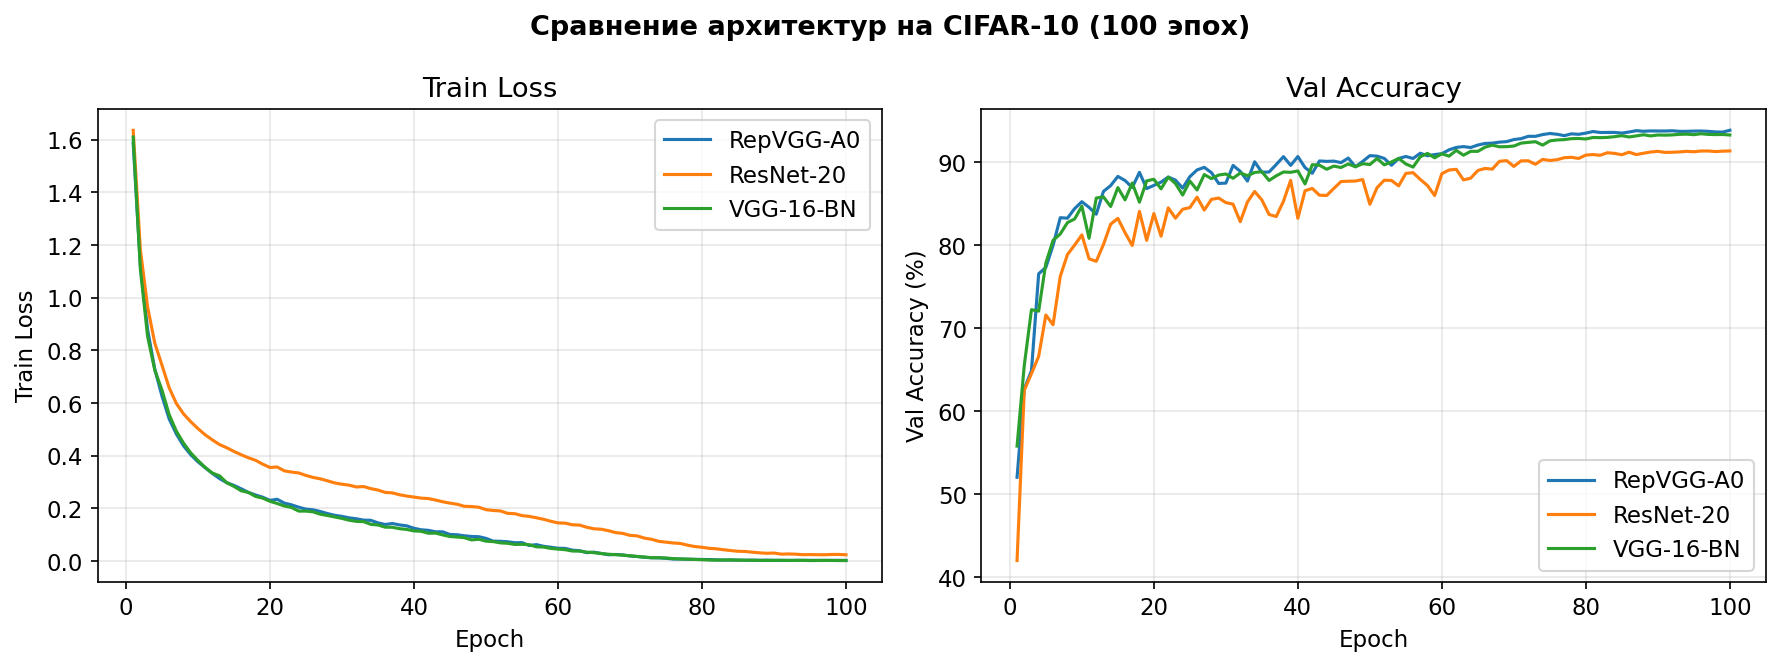
\includegraphics[width=\linewidth]{figures/training_curves.png}
\caption{Динамика обучения трёх моделей на CIFAR-10}
\label{fig:training}
\end{figure}

RepVGG-A0 достигает \repvggAcc{}\%, опережая ResNet-20 на 2.5~п.п. и VGG-16 на 0.4~п.п. Deploy-версия RepVGG вдвое компактнее VGG-16 (\repvggDeployParams{}M против \vggParams{}M) при меньшем числе FLOPs (\repvggDeployFlops{}M против \vggFlops{}M). ResNet-20 при \resnetParams{}M параметров и \resnetFlops{}M FLOPs показывает \resnetAcc{}\% --- высокий результат для модели такого размера, но уступает RepVGG по accuracy на 2.5~п.п.

Кривые обучения (рис.~\ref{fig:training}) показывают, что RepVGG-A0 и VGG-16 сходятся сравнимо быстро и достигают плато после $\sim\!60$ эпох, тогда как ResNet-20 выходит на свой максимум раньше, но на более низком уровне. У всех трёх моделей наблюдается разрыв между train loss и val accuracy, характерный для обучения без сильной регуляризации: train loss продолжает снижаться, но val accuracy перестаёт расти. Это согласуется с результатами эксперимента~4, где добавление Cutout дополнительно поднимает результат.


\subsection{Эксперимент 3: ablation по веткам}

Архитектура RepVGG удобна для ablation, поскольку три ветки тренировочного блока функционально независимы: identity обеспечивает градиентный поток (аналог skip-connection), ветка $1\times1$ расширяет пространство оптимизации, а $3\times3$ --- основную ёмкость модели. Отключая ветки по одной, можно изолировать вклад каждой из них.

RepVGG-A0 обучена в четырёх конфигурациях по 100 эпох:

\begin{table}[H]
\centering
\caption{Ablation: влияние отдельных веток (100 эпох)}
\label{tab:ablation}
\begin{tabular}{@{}lr@{}}
\toprule
Конфигурация & Val Acc (\%) \\
\midrule
$3\times3$ + $1\times1$ + identity (полная) & \ablFull{} \\
$3\times3$ + $1\times1$ (без identity) & \ablNoId{} \\
$3\times3$ + identity (без $1\times1$) & \ablNoOne{} \\
Только $3\times3$ & \ablOnlyThree{} \\
\bottomrule
\end{tabular}
\end{table}

Полная модель (\ablFull{}\%) опережает все усечённые конфигурации: без identity -- \ablNoId{}\%, без $1\times1$ -- \ablNoOne{}\%, только $3\times3$ -- \ablOnlyThree{}\%. Разница составляет 0.3--0.6~п.п. Наибольший вклад вносит ветка $1\times1$ (её удаление снижает результат на 0.6~п.п.), что согласуется с гипотезой авторов о неявной регуляризации через расширение пространства оптимизации.

Конфигурация <<только $3\times3$>> (\ablOnlyThree{}\%) показала результат чуть выше, чем <<без $1\times1$>> (\ablNoOne{}\%). Разница 0.09~п.п. находится в пределах стохастического разброса одиночных запусков, поэтому мы не делаем из этого содержательных выводов.

\begin{figure}[H]
\centering
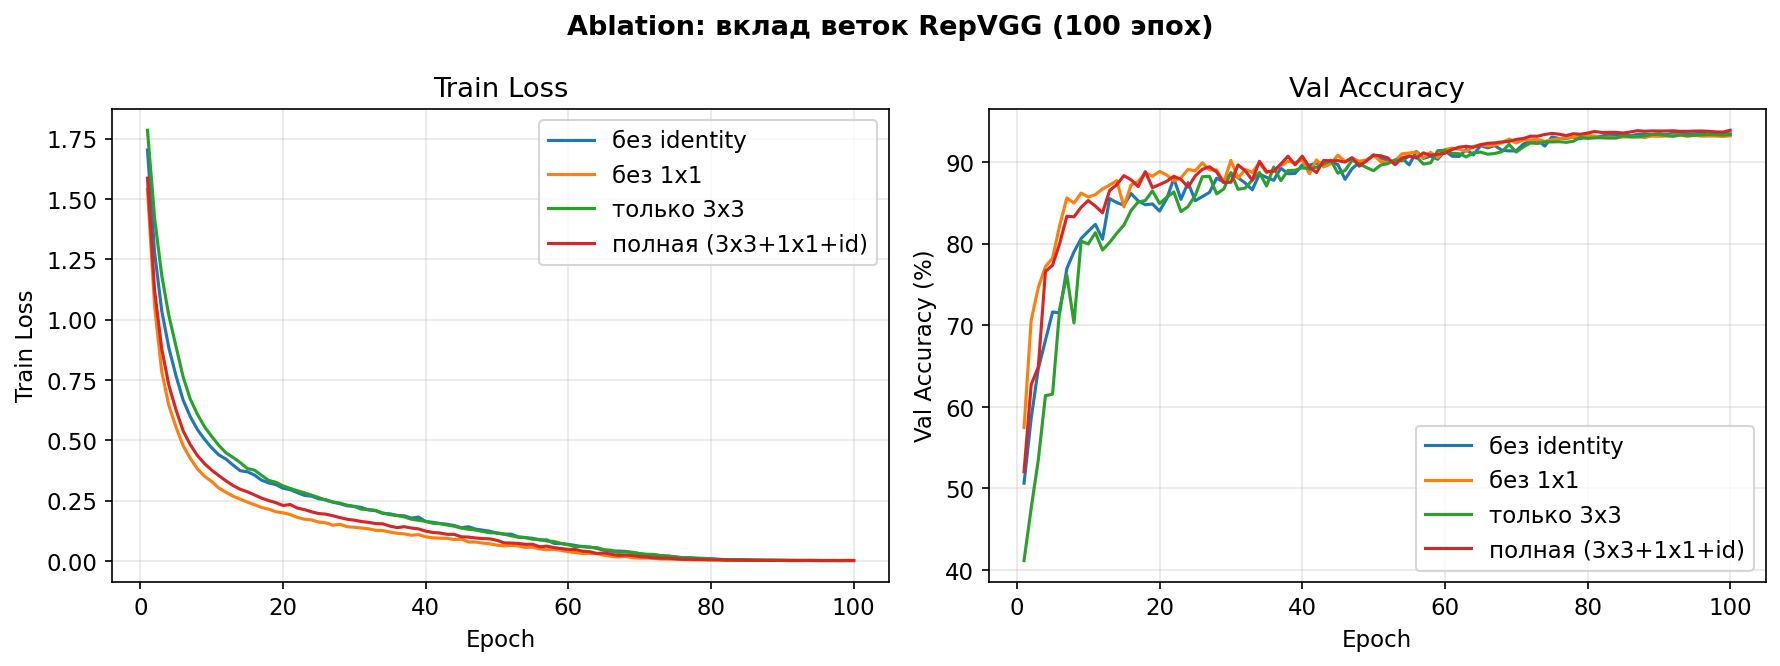
\includegraphics[width=\linewidth]{figures/ablation.png}
\caption{Кривые обучения для разных конфигураций RepVGG (100 эпох)}
\label{fig:ablation}
\end{figure}


\subsection{Эксперимент 4: влияние Cutout}

Cutout~[4] случайно маскирует квадрат $16\times16$ во входном изображении, вынуждая модель использовать пространственно распределённые признаки. RepVGG не содержит встроенных механизмов регуляризации типа Dropout между свёртками, поэтому внешняя регуляризация через аугментации особенно актуальна.

За 100 эпох RepVGG-A0 с Cutout достигает \cutoutAcc{}\% против \ablFull{}\% без Cutout (+1~п.п.). Cutout даёт лучший результат среди всех конфигураций, подтверждая чувствительность plain-архитектур к внешней регуляризации.

\begin{figure}[H]
\centering
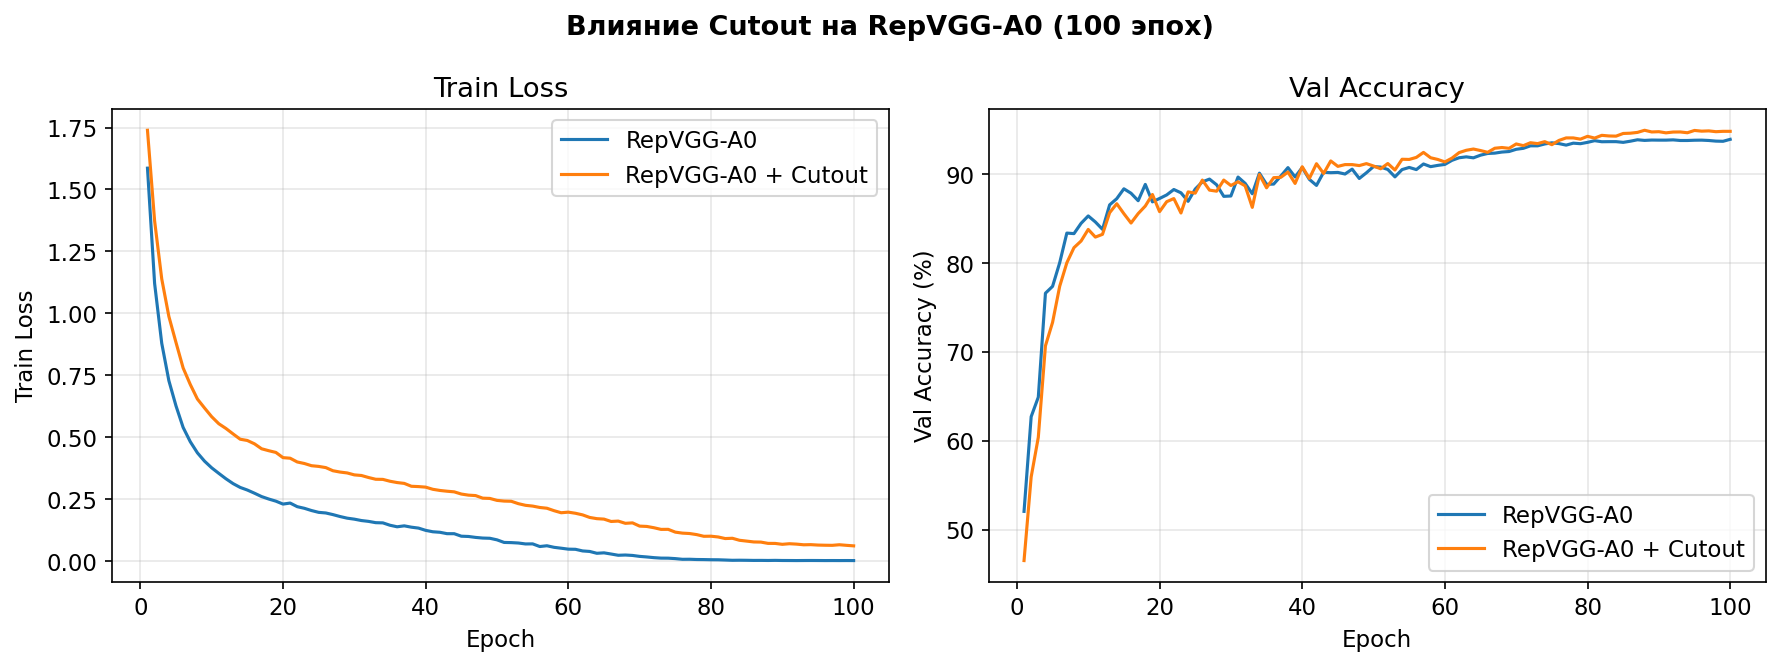
\includegraphics[width=\linewidth]{figures/cutout.png}
\caption{Влияние Cutout на RepVGG-A0 (100 эпох)}
\label{fig:cutout}
\end{figure}

%______________________________________________________
% ЗАКЛЮЧЕНИЕ

\section{Заключение}

Репараметризация RepVGG корректна: разница выходов train- и deploy-версии составляет $\sim\!10^{-6}$. Deploy-модель в \repvggSpeedup{}x быстрее при полном сохранении accuracy.

На CIFAR-10 RepVGG-A0 (\repvggAcc{}\%) превосходит ResNet-20 (\resnetAcc{}\%) и VGG-16 (\vggAcc{}\%), оставаясь вдвое компактнее VGG-16 в deploy-режиме.

Ablation подтвердил вклад каждой ветки: полная модель опережает усечённые на 0.3--0.6~п.п. Наибольший эффект даёт ветка $1\times1$. Cutout поднимает accuracy до \cutoutAcc{}\% (+1~п.п.), подтверждая чувствительность plain-архитектур к внешней регуляризации. Сводные результаты приведены в таблице~\ref{tab:summary}.

\begin{table}[H]
\centering
\caption{Сводка результатов всех экспериментов}
\label{tab:summary}
\begin{tabular}{@{}llr@{}}
\toprule
Эксперимент & Конфигурация & Val Acc (\%) \\
\midrule
\multirow{2}{*}{1. Репараметризация} & Train (multi-branch) & \repvggAcc{} \\
 & Deploy (single-path, \repvggSpeedup{}x быстрее) & \repvggAcc{} \\
\midrule
\multirow{3}{*}{2. Архитектуры} & RepVGG-A0 (deploy) & \repvggAcc{} \\
 & VGG-16-BN & \vggAcc{} \\
 & ResNet-20 & \resnetAcc{} \\
\midrule
\multirow{4}{*}{3. Ablation} & Полная ($3\times3$+$1\times1$+id) & \ablFull{} \\
 & Без identity & \ablNoId{} \\
 & Без $1\times1$ & \ablNoOne{} \\
 & Только $3\times3$ & \ablOnlyThree{} \\
\midrule
4. Cutout & RepVGG-A0 + Cutout & \cutoutAcc{} \\
\bottomrule
\end{tabular}
\end{table}

Ограничения работы: (1)~все эксперименты проведены на CIFAR-10 ($32\times32$) - на ImageNet ($224\times224$) выигрыш от простой deploy-архитектуры был бы значительнее из-за большего объёма свёрточных вычислений; (2)~обучение 100 эпох при стандарте 200--300 для CIFAR --- при более длительном обучении accuracy всех моделей была бы выше; (3)~результаты получены из одного запуска с фиксированным seed, без оценки дисперсии по нескольким seed'ам.

Возможные направления развития: воспроизведение на ImageNet для оценки ускорения на реальных задачах, ablation по объёму данных (обучение на 10--50\% выборки) для проверки устойчивости архитектуры, и сравнение с более поздними методами репараметризации (RepOptimizer, DBB).

%______________________________________________________
% СПИСОК ИСТОЧНИКОВ

\clearpage
\begin{center}
\textbf{СПИСОК ИСТОЧНИКОВ}
\end{center}

\begingroup
\setlength{\parindent}{0pt}
\setlength{\parskip}{1.2em}

[1] Ding X., Zhang X., Ma N., Han J., Ding G., Sun J. RepVGG: Making VGG-style ConvNets Great Again // Proceedings of the IEEE/CVF CVPR. -- 2021.
Режим доступа: \texttt{https://arxiv.org/abs/2101.03697} (дата обращения: 28.03.2026).

[2] He K., Zhang X., Ren S., Sun J. Deep Residual Learning for Image Recognition // IEEE/CVF CVPR. -- 2016.

[3] Simonyan K., Zisserman A. Very Deep Convolutional Networks for Large-Scale Image Recognition // ICLR. -- 2015.

[4] DeVries T., Taylor G.W. Improved Regularization of Convolutional Neural Networks with Cutout // arXiv:1708.04552. -- 2017.

[5] Ioffe S., Szegedy C. Batch Normalization: Accelerating Deep Network Training by Reducing Internal Covariate Shift // ICML. -- 2015.

\endgroup

\clearpage
%______________________________________________________
% ПРИЛОЖЕНИЕ

\appendix
\section*{ПРИЛОЖЕНИЕ}
\addcontentsline{toc}{section}{Приложение}

\subsection*{А. Гиперпараметры обучения}

\begin{table}[H]
\centering
\caption{Полная конфигурация обучения (единая для всех моделей)}
\label{tab:hyperparams}
\begin{tabular}{@{}ll@{}}
\toprule
Параметр & Значение \\
\midrule
SGD: lr / momentum / weight decay & 0.1 / 0.9 / $10^{-4}$ \\
Scheduler & Cosine annealing, $\eta_{\min} = 10^{-6}$ \\
Warmup & 5 эпох (линейный) \\
Эпох / batch size & 100 / 128 \\
Mixed precision & FP16 (torch.amp) \\
RandomCrop / HorizontalFlip & $32\times32$ pad$\,=\,$4 / $p = 0.5$ \\
Cutout (эксп.~4) & $16\times16$ \\
Нормализация & $\mu\!=\!(0.491, 0.482, 0.447)$, $\sigma\!=\!(0.247, 0.243, 0.262)$ \\
\bottomrule
\end{tabular}
\end{table}

\subsection*{Б. Архитектуры базовых моделей}

\begin{table}[H]
\centering
\caption{Базовые модели, адаптированные под CIFAR}
\label{tab:baselines_arch}
\begin{tabular}{@{}lll@{}}
\toprule
Модель & Структура & Парам. / FLOPs \\
\midrule
ResNet-20~[2] & BasicBlock $\times 3$ (16, 32, 64 кан.), GAP + FC & \resnetParams{}M / \resnetFlops{}M \\
VGG-16-BN~[3] & 13 conv $3\times3$ + BN (64\,...\,512 кан.), GAP + FC & \vggParams{}M / \vggFlops{}M \\
\bottomrule
\end{tabular}
\end{table}

\subsection*{В. Исходный код и логи}

\noindent
Репозиторий: \url{https://github.com/Vlasikq/cv_repvgg}\\
Логи экспериментов: \url{https://wandb.ai/vefulls-/RepVGG}

\end{document}
